\documentclass[tikz]{standalone}
\usepackage{bm}
\usepackage{stix}

\usetikzlibrary{calc}

\definecolor{mplblue}{HTML}{1f77b4}
\definecolor{mplorange}{HTML}{ff7f0e}
\definecolor{mplgreen}{HTML}{2ca02c}
\definecolor{mplmagenta}{HTML}{e377c2}

\tikzstyle{site}=[rectangle, minimum width=1.5cm, minimum height=0.75cm, inner sep=0pt, draw=mplblue!80!black, fill=mplblue!20!white]
\tikzstyle{annot}=[inner sep=2pt]

\newcommand{\arr}[1]{{\bm{#1}}}

\begin{document}
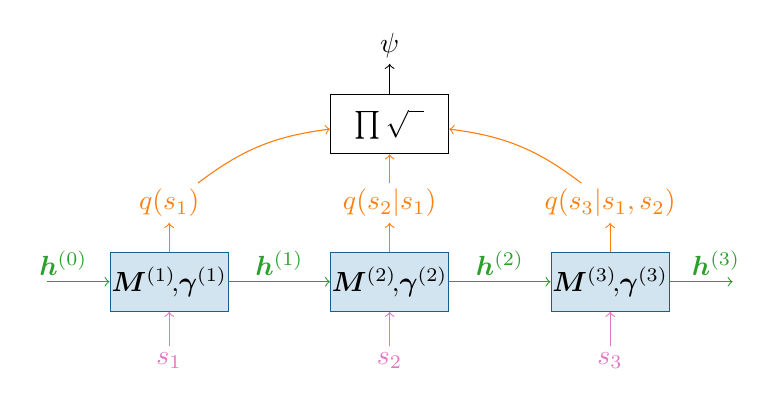
\begin{tikzpicture}[x=2.8cm, y=1cm]

\node (Mm) at (-0.6, 0) {};
\node [site] (M0) at (0, 0) {$\arr{M}^{(1)}\!,\!\arr{\gamma}^{(1)}$};
\node [site] (M1) at (1, 0) {$\arr{M}^{(2)}\!,\!\arr{\gamma}^{(2)}$};
\node [site] (M2) at (2, 0) {$\arr{M}^{(3)}\!,\!\arr{\gamma}^{(3)}$};
\node (M3) at (2.6, 0) {};

\node [site, draw=black, fill=white] (prod) at ($(M1) + (0, 2)$) {$\prod \sqrt{\phantom{x}}$};

\node [annot, above, mplgreen] (hm) at ($(Mm)!.2!(M0)$) {$\arr{h}^{(0)}$};
\node [annot, above, mplgreen] (h0) at ($(M0)!.5!(M1)$) {$\arr{h}^{(1)}$};
\node [annot, above, mplgreen] (h1) at ($(M1)!.5!(M2)$) {$\arr{h}^{(2)}$};
\node [annot, above, mplgreen] (h2) at ($(M2)!.8!(M3)$) {$\arr{h}^{(3)}$};

\node [annot, mplmagenta] (si0) at ($(M0) + (0, -1)$) {$s_1$};
\node [annot, mplmagenta] (si1) at ($(M1) + (0, -1)$) {$s_2$};
\node [annot, mplmagenta] (si2) at ($(M2) + (0, -1)$) {$s_3$};

\node [annot, mplorange] (p0) at ($(M0) + (0, 1)$) {$q(s_1)$};
\node [annot, mplorange] (p1) at ($(M1) + (0, 1)$) {$q(s_2 | s_1)$};
\node [annot, mplorange] (p2) at ($(M2) + (0, 1)$) {$q(s_3 | s_1, s_2)$};

\node [annot] (psi) at ($(prod) + (0, 1)$) {$\psi$};

\draw [->, mplgreen] (Mm) -- (M0);
\draw [->, mplgreen] (M0) -- (M1);
\draw [->, mplgreen] (M1) -- (M2);
\draw [->, mplgreen] (M2) -- (M3);

\draw [->, mplmagenta] (si0) -- (M0);
\draw [->, mplmagenta] (si1) -- (M1);
\draw [->, mplmagenta] (si2) -- (M2);

\draw [->, mplorange] (M0) -- (p0);
\draw [->, mplorange] (M1) -- (p1);
\draw [->, mplorange] (M2) -- (p2);

\draw [->, mplorange] (p0) to [bend left=15] (prod);
\draw [->, mplorange] (p1) -- (prod);
\draw [->, mplorange] (p2) to [bend right=15] (prod);

\draw [->] (prod) -- (psi);

\end{tikzpicture}
\end{document}
